\documentclass[14pt]{extreport}
\usepackage{gost}
\usepackage{minted}

\addto\captionsrussian{\def\refname{Список используемой литературы}}

\begin{document}

\includepdf[pages={1}]{titulnyy_list_oznakomitelnaya_praktika.pdf}


\tableofcontents

\intro

Для современного математика и исследователя важны не только навыки решения задач аналитически и численно на бумаге или доске, но также и умение пользоваться современными пакетами компьютерной алгебры, такими как Euler Math Toolbox или Mathcad, а также умение представить полученные результаты  в определенном стиле и формате. Определенным стандартом оформления работы математика де-факто является издательская система LaTeX.     

В данной работе я получаю практические навыки по двум направлениям, востребованным в современных условиях: использование пакета компьютерной алгебры на примере Euler Math Toolbox, а также верстка математического текста, используя издательскую систему LaTeX. В качестве источника задач мною выбрано издание <<Конспект лекций по высшей математике: полный курс>>  Д. Т. Письменный. - 4-е изд. - М.: Айрис-пресс, 2006. - 608 с.: ил. - (Высшее образование).





\chapter{HTML: База}

\section{HTML}

HyperText Markup Language (гипертекст маркап лэнгуидж) - язык разметки гипертекста. В этой аббревиатуре нам интересно слово "разметка".

Разметка - что это вообще такое? Представь, что ты передаёшь текст по сети. Как сделать в тексте заголовок? Выделить абзац? Подчеркнуть слово? Самый простой вариант - пометить начало и конец выделяемого фрагмента условными метками. Например:
\begin{minted}{HTML}
<заголовок>HTML</заголовок>
<полужирный>HyperText Markup Language</полужирный> <курсив>(гипертекст маркап лэнгуидж)</курсив> - язык разметки гипертекста.
\end{minted}
Это разметка.




\section{Теги}
Тег — это синтаксическая единица языка HTML, которая выделяет или создаёт элемент. Это набор символов, с помощью которого браузер понимает, где элемент создается, начинается и заканчивается. Есть 2 вида тегов: двойные и одинарные.

Двойные теги
Двойные теги показывает начало и конец элемента. Начало элемента обозначается открывающим тегом \mintinline{latex}{<…>}, а конец - закрывающим \mintinline{latex}{</…>}.

Двойной тег обязательно должен быть закрыт. Даже несмотря на то, что современные браузеры умеют в некоторых случаях понимать разметку без закрытых тегов, лучше всегда закрывать их.

Одинарные теги
Одинарные теги просто не имеют пары. Примеры: тег переноса строки \mintinline{latex}{<br>} или горизонтальной линии  \mintinline{latex}{<hr>}.

Старые браузеры требовали закрывать одинарные теги: \mintinline{latex}{<br />}, сейчас таких браузеров практически не осталось и допустимо использовать оба варианта синтаксиса.



\section{Атрибуты}
Атрибуты — это свойства тега. С помощью них мы задаём параметры тега.

Сразу возьмём пример: тег \mintinline{latex}{<a>} — ссылка. Для задания адреса, куда будет вести эта ссылка, нам понадобится атрибут \mintinline{latex}{href}. Вот так будет выглядеть ссылка на страницу ITC Вконтакте:
\begin{minted}{html}
<a href="https://vk.com/itc.digital">ITC Вконтакте</a>
\end{minted}
Атрибут указывается внутри тега, значение атрибута указывается внутри кавычек. Атрибуты отделяются друг от друга пробелами. Пример ссылки на страницу ITC, которая откроется в новой вкладке:

\begin{minted}{html}
<a href="https://vk.com/itc.digital" target="_blank">ITC Вконтакте</a>
\end{minted}

У атрибута может не быть значения, тогда наличие атрибута включает какой-то параметр, а отсутствие - отключает. Например, атрибут \verb disabled. Если кнопке \mintinline{latex}{<button>} задать атрибут \mintinline{latex}{disabled}, она станет серой и на неё невозможно будет нажать.

\begin{minted}{html}
<button disabled>Нельзя нажимать</button>
\end{minted}

\begin{figure}[H]
\centerline{
\includegraphics[width=0.5\linewidth]{pics_practice/disabled_button.png}}
\caption{}
\label{1}
\end{figure}




\section{Особенности интерпретации HTML}

\emph{Перенос строки только через тег.}

Возможно, у тебя возник вопрос, зачем нужен тег переноса строки, если можно просто нажать энтер. Дело в том, что HTML воспринимает перенос строки как пробел. Это нужно потому, что редакторы кода не переносят строки, которые не помещаются в экран - так удобнее писать код. Поэтому чтобы длинный текст влезал в экран, в коде ставятся переносы строки, которые не нужны, когда страница показывается в браузере.

\emph{Несколько пробелов, идущих подряд, считаются за один.}

Это происходит по той же причине, что и с переносом строки. Так просто удобнее форматировать код в редакторе. Из-за того, что теги вкладываются друг в друга, для удобного восприятия кода вложенность показывают отступами - пробелами. Пример:

\begin{figure}[H]
\centerline{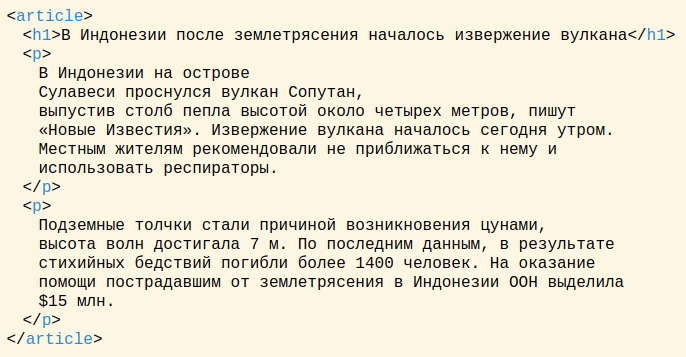
\includegraphics[width=0.8\linewidth]{pics_practice/interpretation_HTML.png}}
\caption{}
\label{2}
\end{figure}

\emph{Произвольный регистр.}

\mintinline{latex}{<br>} даст такой же результат, что и \mintinline{latex}{<BR>}, и \mintinline{latex}{<Br>}, и \mintinline{latex}{<bR>}. Несмотря на это, писать разметку лучше в нижнем регистре - это негласное правило.

\emph{Перенос строки в теге.}

При определении тега и его атрибутов можно переносить строку. Это полезно для длинных определений.
Например, для этого изображения:
\begin{minted}{html}
<img
  src="http://example.com/cat.jpg"
  title="Мурка"
  alt="Рыжая кошка валяется в снегу"
  width="640"
  height="480"
>
\end{minted}





\chapter{HTML: Основные элементы}

\section{Структура HTML-документа}

Структура HTML документа - скелет, на основе которого строится вся страница:
\begin{minted}{html}
<!DOCTYPE html>
<html>
  <head>
    <meta charset="utf-8">
    <title>Страница</title>
  </head>
  <body>
    <h1>...</h1>
    <p>...</p>
  </body>
</html>
\end{minted}

\textbf{<!DOCTYPE>}

Первым тегом в любом HTML документе должен идти тег <!DOCTYPE>. Он говорит браузеру, по какому стандарту написана страница. На рассвете веба HTML существовал в разных несовместимых версиях, поэтому для их одновременной поддержки нужно было указывать версию явно. Сейчас все пришли к одному стандарту - HTML5. Поэтому для всех сайтов, которые создаются сегодня, нужно указывать <!DOCTYPE html> - так обозначается HTML5.

\textbf{<html>}

Вторым тегом идет <html> - контейнер, который содержит два тега - \mintinline{latex}{<head>} и \mintinline{latex}{<body>}. HTML-страница должна заканчиваться закрытым тегом \mintinline{latex}{</html>}.

\textbf{<head>}

В теге <head> хранится информация о странице. Здесь указывают кодировку \mintinline{latex}{<meta charset="...">}, имя страницы \mintinline{latex}{<title>...</title>}, специальную информацию для поисковиков, а ещё тут подключаются стилевые файлы и скрипты.

Тег \mintinline{latex}{<head>} не отображается. Его цель — сказать браузеру информацию о странице.

\textbf{<body>}

В теге \mintinline{latex}{<body>} размещается весь контент страницы, который пользователь увидит в браузере.





\section{Практика: создание веб-страницы}
Создаем файл и называем его \textbf{index.html}. Вставляем туда структуру HTML-страницы из предыдущего урока:
\begin{figure}[H]
\centerline{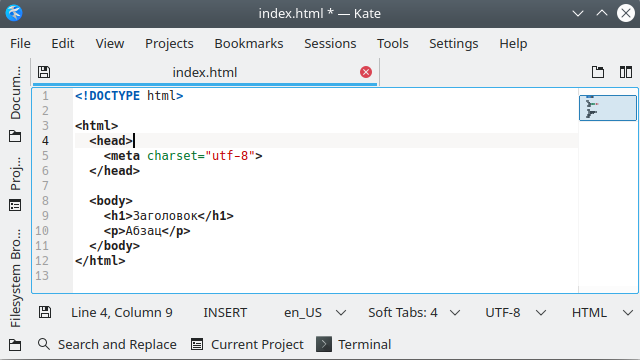
\includegraphics[width=0.8\linewidth]{pics_practice/index_html.png}}
\caption{}
\label{3}
\end{figure}
Сохраняем файл и открываем в браузере. Видим:
\begin{figure}[H]
\centerline{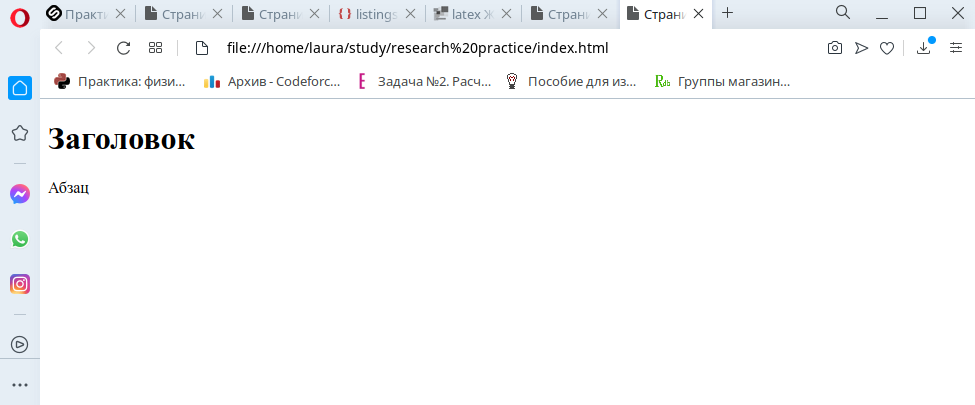
\includegraphics[width=0.8\linewidth]{pics_practice/header.png}}
\caption{}
\label{4}
\end{figure}




\section{Редакторы кода}

Разработчики пишут код в специальных редакторах. Они отличаются назначением. Остальные отличия почти всегда вытекают из него. Существует несколько редакторов кода, которые подходят для веб-разработки. Мы рассмотрим несколько из них и порекомендуем два (один из них только для слабых компьютеров). 
Notepad++ - для ветеранов.
Боевая классика. Ветеран среди редакторов кода, в бородатые года считался самым популярным у веб-разработчиков. Сегодня его в основном используют ностальгирующие консерваторы.

Sublime Text -  для слабых компьютеров.
Самый популярный редактор кода у разработчиков на Python. Для веб-разработки тоже подходит. Довольно быстро работает, неплохо выглядит и кастомизируется, имеет несколько полезных плагинов. В целом неплох, но для веб-разработчика есть более подходящий софт. Рекомендуем использовать его только если у тебя слабый компьютер.

Atom - для хипстеров.
Хороший редактор кода, заточенный под веб-разработку. Много тем оформления, плагинов. Работает на веб-технологиях, поэтому если ты планируешь развиваться дальше и изучать JavaScript, то в дальнейшем сможешь писать свои расширения. Его минус - скорость работы. Поэтому его использовать не рекомендуем.

Visual Studio Code - рекомендация.
Не путай с Visual Studio. Редактор кода для веба от Microsoft. По сути, это более быстрый аналог Atom. Он имеет все те же самые плюсы, что и Atom, но работает ощутимо быстрее. Из минусов только майкрософтовый тоталитарный внешний вид, который легко изменить, установив другую тему оформления.



\section{Элементы и их виды}

Элементы - то, что создаётся тегами. Можно сказать, что теги это текстовое представление элементов. Элементы бывают двух видов:

\emph{Блочные элементы}

Составляют структуру страницы.

Особенности:
\begin{itemize}
\itemблоки располагаются друг под другом по вертикали
\itemзапрещено вставлять блочный элемент внутрь строчного
\itemзанимают всё допустимое пространство по ширине
\itemвысота вычисляется автоматически, исходя из содержимого
\end{itemize}

Примеры:
\begin{itemize}
\itemабзацы \mintinline{latex}{<р>}
\itemсписки: маркированные (с маркером) \verb <ul> и нумерованные (с числами) \mintinline{latex}{<ol>}
\itemзаголовки: от первого уровня \verb <h1> до шестого уровня \mintinline{latex}{<h6>}
\itemстатьи \mintinline{latex}{<article>}
\itemразделы \mintinline{latex}{<section>}
\itemдлинные цитаты \mintinline{latex}{<blockquote>}
\itemблоки общего назначения  \mintinline{latex}{<div>}
 \end{itemize}

\emph{Строчные элементы}

Используются для форматирования текстовых фрагментов. Обычно содержат одно или несколько слов.

Особенности:
\begin{itemize}
\itemэлементы, идущие подряд, располагаются на одной строке и переносятся на другую при необходимости
\itemвнутрь допустимо вставлять текст или другие строчные элементы, помещать блочные элементы - запрещено
\end{itemize}

Примеры:
\begin{itemize}
\itemссылки \mintinline{latex}{<a>}
\itemвыделенные слова \mintinline{latex}{<em>}
\itemважные слова \mintinline{latex}{<strong>}
\itemкороткие цитаты \mintinline{latex}{<q>}
\itemаббревиатуры \mintinline{latex}{<abbr>}
\end{itemize}




\section{Списки}

В HTML существует три вида списков:

\emph{Маркированный}

Список из неупорядоченных элементов.

Состоит из двух тегов:
\begin{itemize}
\item \verb <ul> (unordered list) - тег начала и конца списка
\item \verb <li> (list item) - пункт списка
\end{itemize}

Пример:

\begin{minted}{html}
Список ингредиентов:
<ul>
     <li>Картошка</li>
     <li>Морковка</li>
     <li>Свекла</li>
</ul>
\end{minted}




\section{Изображения}

Для добавления изображения используется тег \verb <img>. Это одинарный тег. Вот его основные атрибуты:

\begin{itemize}
\item \verb src - ссылка на картинку;
\item \verb alt - текст, который отображается вместо картинки, если она не загрузилась;
\item \verb title - текст, который отображается при наведении мыши на картинку;
\item \verb width - ширина картинки в пикселях;
\item \verb height - высота картинки в пикселях;
\end{itemize}

Пример:
\begin{minted}{html}
<img
    src="http://example.com/cat.jpg"
    title="Мурка"
    alt="Рыжая кошка валяется в снегу"
    width="640"
    height="480"
>
\end{minted}

Семантичные изображения с подписью в HTML 5
В HTML 5 появились теги для оформления объектов с подписями - \verb figure  и \verb figcaption. Если твоей картинке нужна подпись - пользуйся ими. Пример кода:
\begin{minted}{html}
<figure>
  <img src="https://www.google.ru/images/branding/googlelogo/2x/googlelogo_color_120x44dp.png">
  <figcaption>
    Лого гугла от 2015 года
  </figcaption>
</figure>
\end{minted}
Результат:
\begin{figure}[H]
\centerline{
\includegraphics[width=0.4\linewidth]{pics_practice/google.png}}
\caption{}
\label{5}
\end{figure}


\section{Ссылки и адреса}

Мы уже знакомы со ссылками:
\begin{minted}{html}
<a href="https://google.com/">Google</a>
\end{minted}
Повторим: для создания ссылки необходимо использовать тег \verb <a>. Атрибут \verb href  указывает адрес, по которому будет совершён переход.

Адреса бывают двух видов:

\emph{Абсолютные адреса}

Абсолютный адрес, записанный в полной форме. Например,
\begin{minted}{html}
https://google.com/doodles
\end{minted}
Давай разберём этот адрес:
\begin{itemize}
\item \verb https - так называемая «схема», обычно это название протокола. HTTPS - защищённая версия HTTP;
\item \verb google.com - доменное имя сайта;
\item \verb /doodles - путь (директория) внутри сайта;
\end{itemize}

\emph{Относительные адреса}

Относительный - сокращённый адрес. В таком адресе начальная часть опущена и браузер использует текущий адрес для определения полного адреса. Примеры:
\begin{itemize}
\item//google.com - ссылка на домен в текущем протоколе: если мы находимся по адресу, который начинается с http, то ссылка будет вести на http://google.com
\item/sheets - ссылка на путь внутри текущего домена: если мы находимся на http://google.com, то ссылка будет вести на http://google.com/sheets, а если на http://facebook.com, то на http://facebook.com/sheets.
\item page2 - ссылка на путь внутри текущей директории: если мы находимся на http://site.com/routes/page1, то попадём на http://site.com/routes/page2
\end{itemize}




\chapter{HTML: Составные элементы}

\section{Таблицы}

Таблицы в HTML создаются при помощи тега \mintinline{latex}{<table>}.

Внутри него размещают строки таблицы \mintinline{latex}{<tr>} (table row).

Внутри строк помещают ячейки строки \mintinline{latex}{<td>} (table data).

Тегом \verb <th> (table header) размечаются заголовочные ячейки. Он отличается от  \verb <td>  тем, что его содержимое будет выделено полужирным и выровнено по центру.
Существует возможность группировать строки таблицы тегами \verb <thead>, \verb <tfoot>, \verb <tbody>. Они не являются обязательными, но их рекомендуется использовать. Они дают частям таблицы семантический смысл.
\begin{itemize}
\item \verb <thead> - для заголовка,
\item \verb <tfoot> - нижний колонтитул таблицы,
\item \verb <tbody> - основной контент таблицы.
\end{itemize}
Интересный факт: \verb <tfoot>  в коде можно расположить перед \verb <tbody>  или после него, но браузеры всегда выводят его в конце таблицы.

\verb <thead>  и \verb <tfoot>  можно использовать только по одному разу в одной таблице, а количество \verb <tbody>  может быть любым. С помощью нескольких \verb <tbody>  можно разделить контент таблицы на смысловые части. Например, так в таблице могут быть представлены данные за несколько лет, и каждый год будет вынесен в отдельный \mintinline{latex}{<tbody>}.

Название таблицы можно разместить в теге \verb <caption>. Этот тег располагают внутри тега \verb <table>  в самом начале, перед тегами \verb <thead>, \mintinline{latex}{<tfoot>}, \mintinline{latex}{<tbody>}.



\section{Формы}

Формы используются для сбора информации, которую пользователь вводит в специально отведённые поля этой формы. Когда он введёт свои данные и нажмет кнопку «Отправить», все эти данные будут отправлены на сервер. Затем они будут обработаны и сервер отправит ответ пользователю. Существует два основных метода отправки данных: GET и POST.

\textbf{GET}

Когда ты вводишь в адресной строке браузера какой-либо адрес и переходишь по нему, ты отправляешь серверу запрос, называемый GET. В таком запросе данные могут отсутствовать, как здесь: https://www.google.ru/. А вот запрос https://www.google.ru/search?q=itс+stepik содержит в себе переменную q, которая имеет значение itc stepik. В данном случае запрос отправляется на адрес https://www.google.ru/search,  а данные из полей и их названия идут после ? через знак \&. Предварительно данные кодируются в URL код, чтобы сервер не перепутал служебные символы (вроде /, или \&) с частью запроса.

\textbf{POST}

Методом POST так же можно отправлять данные в URL. Но, в отличие от GET, он может иметь тело - специальную "коробочку", в которую можно положить данные, которые уйдут на сервер.

Этот метод обычно используется для отправки форм и загрузки файлов.



\section{Домашнее задание}

Мною было выполнено задание по верстке страницы по макету, со следующими требованиями:
\begin{enumerate}
\item Сверстанная страница обязательно должна быть семантически верной. Если ты сомневаешься в выбранном теге, зайди на сайт оригинала и может так тебе станет яснее: https://ru.wikipedia.org/wiki/Хьюстон
\item Необходимо верстать без использования CSS.
\item В содержании должны быть якоря на все заголовки.
\item Твоя страница может и будет отличаться внешне от макета. Главное - верстка должна быть семантически верной.
\end{enumerate}

\begin{figure}[H]
\centerline{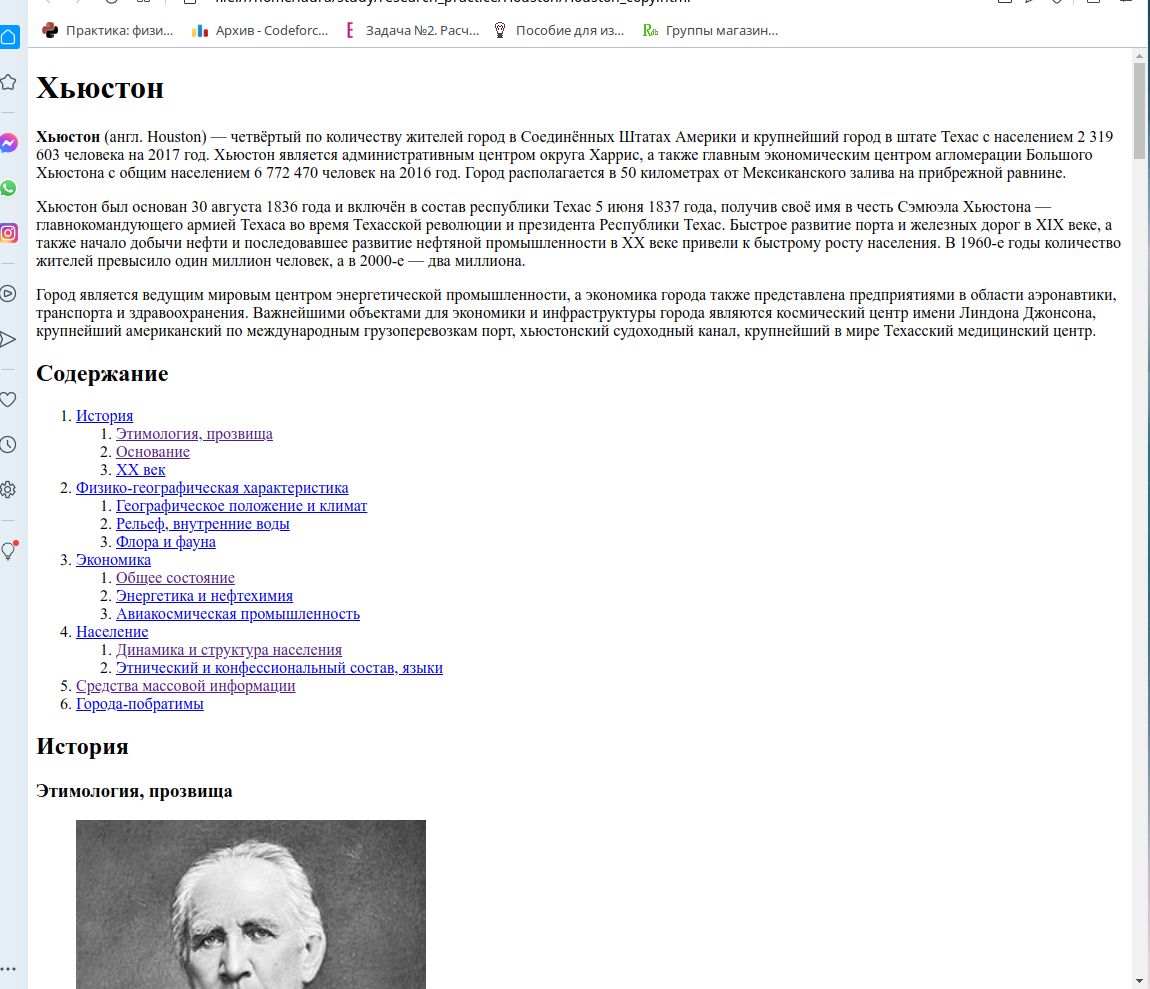
\includegraphics[width=0.7\linewidth]{pics_practice/houston.png}}
\caption{Скриншот страницы}
\label{6}
\end{figure}

Выполненное задание загружено на github.com по адресу https://github.com/laurardaz/Houston




\chapter{CSS: Введение}
\section{Синтаксис CSS}

Синтаксис CSS состоит из двух частей: селекторы и свойства. Селекторами мы указываем элементы, а свойствами описываем их стиль.

\emph{Селекторы}

Селектор это правило, по которому будут выбраны элементы — например, мы можем обратиться ко всем параграфам или картинкам. Как?
\begin{minted}{css}
p {} img {}
\end{minted}

\emph{Свойства}

Свойства пишутся у конкретных селекторов между фигурными скобками в формате ключ: значение.

Сложно? Вот пример как сделать у всех параграфов красный цвет и подчёркивание:
\begin{minted}{css}
p {
    color: red;
    text-decoration: underline;
}
\end{minted}

Каждое новое свойство пишется с новой строки. После каждого свойства необходимо ставить точку с запятой.




\section{Простые селекторы}

HTML-документ состоит из элементов (чем элементы отличаются от тегов, мы рассказали в этом уроке). Чтобы задать стили элементу, необходимо к нему обратиться - «выбрать» его.

Давай посмотрим на примере:
\begin{minted}{css}
<p>Привет, о многоуважаемый ученик!</p>
p {
    color: red;
}
\end{minted}

\begin{figure}[H]
\centerline{
\includegraphics[width=0.5\linewidth]{pics_practice/simple_selector.png}}
\caption{}
\label{7}
\end{figure}

Что мы сделали? Мы раскрасили текст "Привет, о многоуважаемый ученик!" в красный цвет. Как мы это сделали? Мы обратились ко всем элементам \verb <p>  и задали им красный цвет текста. Такой селектор называется селектор по тегу.

Это основные типы селекторов. Есть и более сложные, но их очень редко используют даже опытные разработчики. Потому что один из главных принципов в написании кода - KISS.

\emph{По тегу}

Самый простой селектор - выбирает элементы по их тегу:
\begin{minted}{css}
h1 {
    /* стили для всех h1 */
}
\end{minted}

Этот селектор выберет все элементы \verb <h1> .

\emph{По классу}

Самый часто используемый селектор — по классу. Задаём в HTML класс элементам, к которым применить стиль:
\begin{minted}{css}
<div class="card">
    Карточка
</div>
\end{minted}

И теперь эти элементы можно выбрать по имени класса. Имя селектора начинается с точки:
\begin{minted}{css}
.card {
    /* стили для всех элементов с class="card" */
    background: #333; /* фон серого цвета */
}
\end{minted}

\emph{По id}

Задавать стили по id - дурной тон, старайся его избегать. Тут всё тоже самое, что и с классом, только атрибут называется id:
\begin{minted}{css}
<button id="button-go-to-top">
    Наверх
</button>
\end{minted}
И имя селектора начинается с решётки:
\begin{minted}{css}
#button-go-to-top {
    /* стили для элемента с id="button-go-to-top" */
    text-decoration: underline; /* подчёркивание текста */
}
\end{minted}

\emph{По атрибуту}
 
Не самый популярный селектор, но иногда он полезен:
\begin{minted}{css}
<button data-my-custom-attribute="my-custom-value">
    Нажми на меня
</button>
\end{minted}
 Имя и значение атрибута пишется в квадратных скобках. Работает с любым атрибутом:
\begin{minted}{css}
[data-my-custom-attribute="my-custom-value"] {
    color: red;
}
\end{minted}


\emph{Любой элемент}

Селектор \verb *  выбирает абсолютно любой элемент. Самый непопулярный селектор, обычно используется для костылей. Вряд ли он будет часто тебе нужен. Просто знай, что он есть.
\begin{minted}{css}
* {
    margin: 0;
}
/* абсолютно всем элементам будет установлен margin: 0 */
\end{minted}



\section{Составные селекторы}

Составные селекторы состоят из комбинации простых.

\emph{Группировка селекторов}

Один и тот же набор свойств можно применить к разным селекторам. Пример:
\begin{minted}{css}
button,
.button,
.cta-button {}
\end{minted}
Нужно просто указать  через запятую все селекторы, к которым ты хочешь применить стили.

\emph{Элемент с классом}

Можно стилизовать конкретный элемент, если у него есть определённый класс. Примеры:
\begin{minted}{css}
p.example {}
\end{minted}
Селектор выберет все p, у которых есть класс \verb example .
\begin{minted}{css}
.main.active {}
\end{minted}
Селектор выберет все элементы с классом main, у которых также есть и класс \verb active. Пример такого элемента:
\begin{minted}{css}
<div class="main active">Пример</div>
\end{minted}




\section{Домашнее задание}

Стилизую первое домашнее задание с применением CSS.

Требования:
\begin{enumerate}
\item Контент занимает 70 \% ширины страницы.
\item Контент выровнен по середине.
\item Заголовки всех уровней выполнены шрифтом без засечек.
\item Верхний отступ заголовков установлен больше нижнего (например, 1.5em), чтобы соблюсти правило внутреннего и внешнего.
\item Заголовки первого уровня имеют размер 32px.
\item Таблицы имеют непрерывные границы чёрного цвета толщиной 1px.
\item Подписи под картинками выполены курсивом.
\item Картинки обтекаются текстом. Картинки справа, текст слева.

\end{enumerate}
\begin{figure}[H]
\centerline{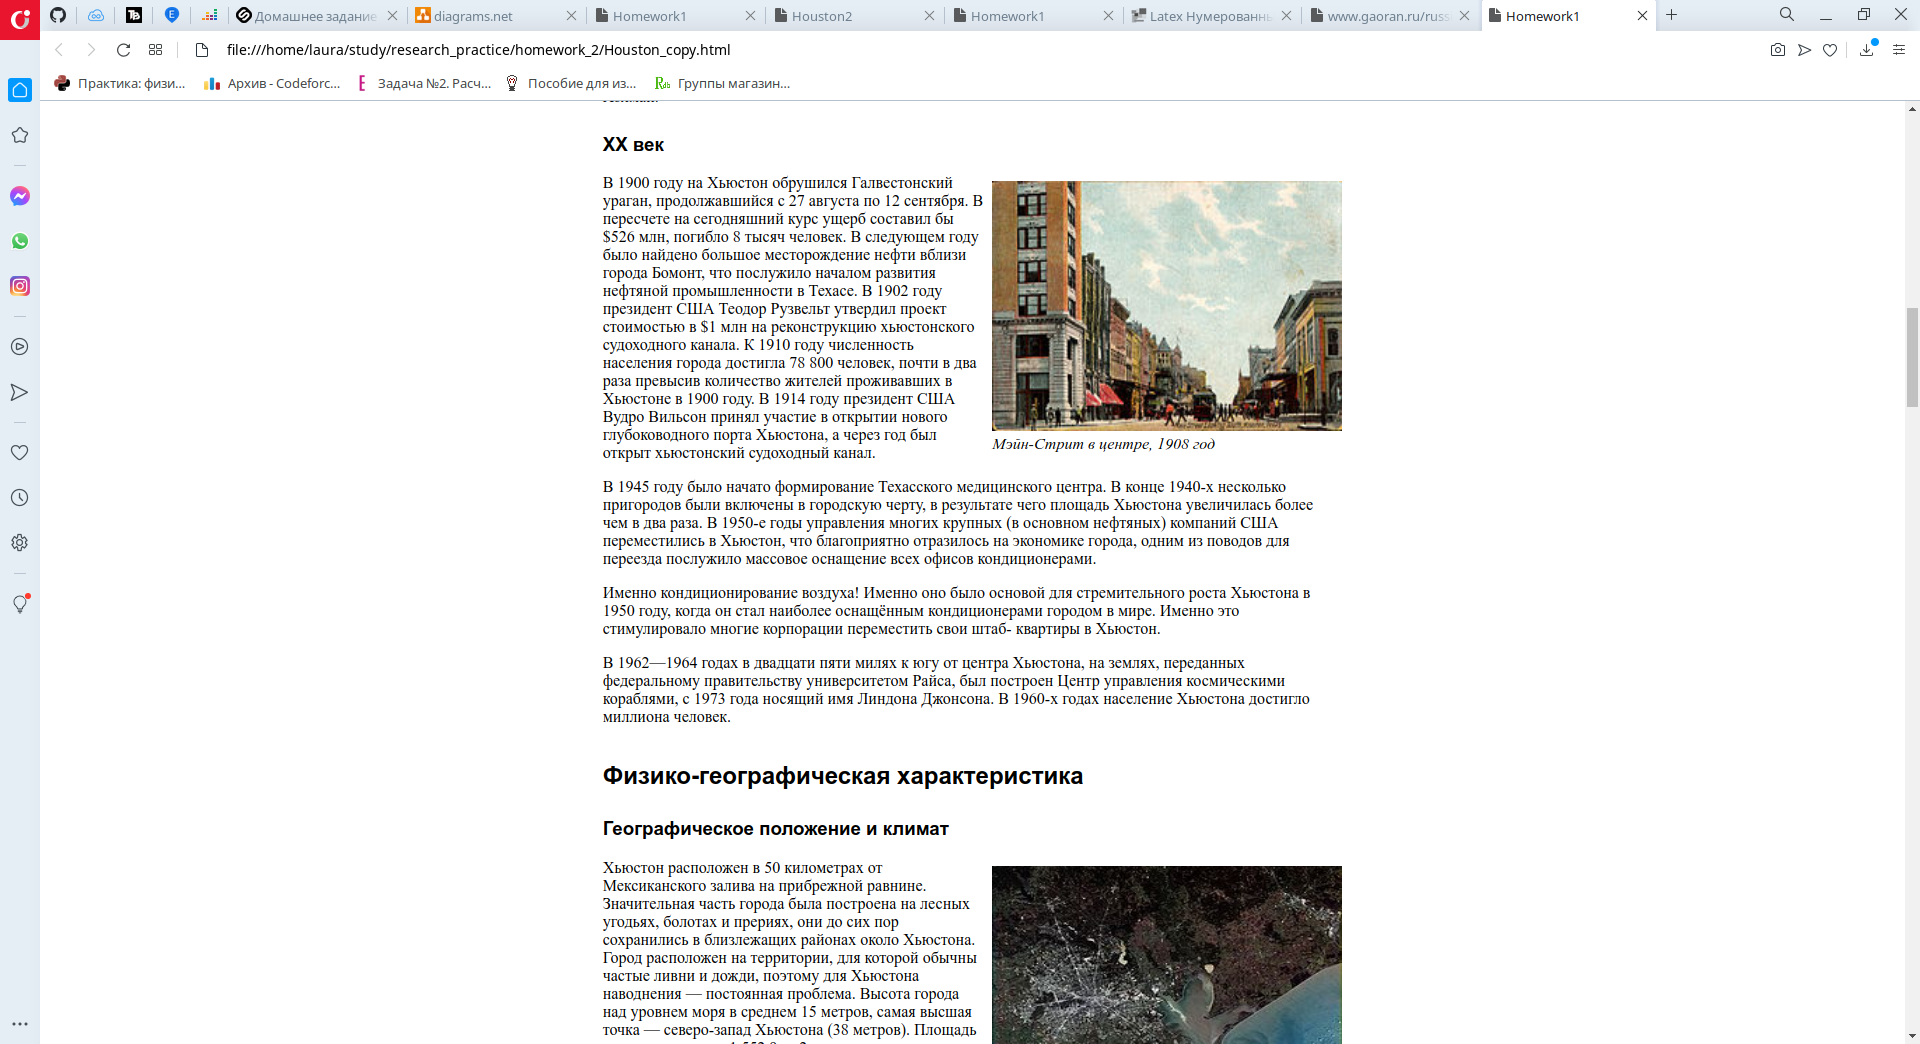
\includegraphics[width=0.8\linewidth]{pics_practice/houston2.png}}
\caption{}
\label{8}
\end{figure}

Выполненное задание загружено на github.com по адресу https://github.com/laurardaz/houston-css





\chapter{CSS: База}

\section{Текст и шрифт}

С помощью CSS можно делать любые операции с текстом и шрифтом. Самые основные действия это:
\begin{itemize}
\item изменение свойств шрифта: семейство, начертание, размер, толщина, стиль и т.д.
\item изменение свойств текста: цвет, расстояние между буквами и строками, подчёркивание/надчёркивание/зачёркивание, выравнивание и т.д.
\end{itemize}
Чтобы узнать, как применить нужный стиль, просто загугли или воспользуйся справочником.





\section{Цвет и фон}

\emph{Фон}

В CSS блокам можно задавать фон. Фоном может быть цвет или картинка. Картинку можно располагать с помощью координат, центрировать, растягивать на весь блок, или задавать в виде повторяющегося бесконечного паттерна. Всё это делается с помощью свойства \verb  background.
Примеры:
\begin{minted}{css}
.example {
   /* цвет фона «продающий красный», задан в HEX-формате */
   background: #e64c0c;
}

.example {
   /* картинка на фоне */
   background: url('images/nude-president.png'); 

   /* background-size отвечает за размер картинки, cover - картинка растягивается на весь блок, сохраняя пропорции */
   background-size: cover;
}
\end{minted}

\emph{Цвет}

Цвет можно ставить не только фону, но и тексту, границам, теням. Есть несколько способов указать цвет:
\begin{itemize}
\item Имя цвета из списка HTML-цветов, например "red", "green", "blue" , "lemonchiffon".
\item HEX, цвет в шестнадцатеричном формате. Начинается с решётки, например \verb #3ae6сa. Можно подобрать с помощью любого color picker'а. Первые шесть символов отвечают за цвет, последние два - необязательные - отвечают за прозрачность. Но прозрачность удобнее задавать через RGBA и HSLA, потому что десятичные дроби удобнее читать и редактировать.
\item RGB (red, green, blue) - цвет, заданый тремя значениями (от 0 до 255) базовых цветов - красного, зелёного и синего. Пример: \verb rbg(255, 123, 13).
\item RGBA - тоже самое, что и RGB, только с прозрачностью, которая задаётся четвёртым числом от 0 до 1, пример: \verb rgba(144, 32, 16, 0.5).
\item HSL, HSLA - цветовая модель, в которой цветовыми координатами являются тон, насыщенность и светлота. Подробнее о ней. HSLA - HSL + прозрачность. Пример: hsl(120, 100\%, 50\%).
\end{itemize}



\section{Домашнее задание}

В этом домашнем задании я научилась работать с макетами. Обычно, когда разработчику поручают сверстать сайт, ему дают макет. Раньше макеты отсылали в PSD (формат фотошопа), а маргинальные дизайнеры вообще давали обычные картинки. Сейчас самый удобный способ передать макет - загрузить файл макета (например, в PSD) в специальный сервис. Там он преобразуется в интерактивный макет, который можно смотреть прямо в браузере. Разработчику нужно просто перейти по ссылке.  будем пользоваться одним из таких сервисов, он называется Figma.








\conclusions

Я достигла целей, которые были поставлены передо мной в данной ознакомительной практике, а именно познакомилась со способами нахождения пределов, производных, а также решением сопутствующих задач в пакете компьютерной алгебры Euler Math Toolbox. Также я овладела принципами верстки в издательской системе LaTeX.  В процессе работы над данным документом я пользовалась официальной документацией, а также навыками решения модельных задач, полученными ранее в курсе математического  анализа. Сложнее всего для меня было освоить синтаксис элементов оформления математического текста в системе LaTeX. Частично мне помог в решении этой проблемы пакет TeXworks с подсветкой синтаксиса.  

Отдельную задачу представляла установка необходимого программного обеспечения в дистрибутиве Linux - Ubuntu 18.04. Файлы с исходным кодом LaTeX я версионировала, используя систему контроля версий git, разместив репозиторий на ресурсе github по адресу https://www.github.com/laurardaz/practice. С помощью этого удалось фиксировать промежуточные версии работы, что сделало нахождение ошибок при верстке легким и быстрым. 

Полученные мной навыки я считаю полезными и перспективными для моего последующего обучения, прохождения практики, а также трудоустройства.  

\newpage
 

 
%далее сам список используевой литературы
\begin{thebibliography}{}
    \bibitem{litlink1}  Письменный Д. Т.  -  "Конспект лекций по высшей метематике: полный курс" - 4-е изд. - М.: Айрис-пресс, 2006.- 608 с.: ил. - (Высшее образование).
    \bibitem{overleaf.com}  LaTeX Basics [Электронный ресурс]. - https://www.overleaf.com/learn
    \bibitem{other-link-name} Euler Math Toolbox Tutorials [Электронный ресурс]. -  http://www.euler-math-toolbox.de/tutorials.html
    \bibitem{overleaf.com}Online LaTeX Editor [Электронный ресурс]. - https://www.overleaf.com/
    \bibitem{overleaf.com}LaTeX:Symbols [Электронный ресурс]. - https://artofproblemsolving.com/wiki/

index.php/LaTeX:Symbols

\end{thebibliography}

\end{document} 
